\documentclass{article}
\usepackage{graphicx}
\usepackage[margin=1.5cm]{geometry}
\usepackage{amsmath}

\begin{document}
\twocolumn

\title{Wednesday Reading Assessment: Unit 6, Circular Motion}
\author{Prof. Jordan C. Hanson}

\maketitle

\section{Memory Bank}

\begin{itemize}
\item $\Delta s = r \Delta \theta$ ... Arc length, radius, and angle (radians)
\item $\omega = \frac{\Delta \theta}{\Delta t}$ ... Definition of angular velocity
\item $v = r\omega $ ... Relationship between tangential velocity, $v$, and angular velocity, $\omega$
\item $C = 2\pi r$ ... Circumference of a circle
\item $a_{\rm C} = r\omega^2$ ... Centripetal acceleration
\item $F_{\rm C} = m r \omega^2$ ... Centripetal force
\end{itemize}

\begin{figure}[ht]
\centering
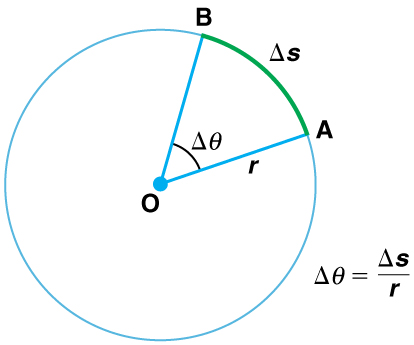
\includegraphics[width=0.3\textwidth]{circle.jpeg}
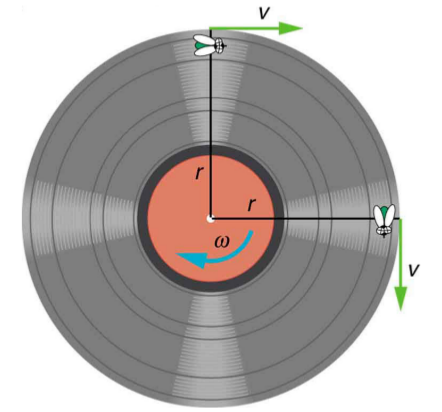
\includegraphics[width=0.25\textwidth]{record.png}
\caption{\label{fig:record} (Left) A circle with a radius $r$.  Arc length $\Delta s$ around the edge is related to the angle $\Delta \theta$.  (Right) A record that is spinning counter-clockwise.}
\end{figure}

\section{Angular Displacement, Velocity}

\begin{enumerate}
\item Suppose disc has a radius of 0.1 m. (a) What is the circumference?  Suppose the object begins to rotate.  A spot on the edge returns to its original location after 1.5 seconds.  (b) Compute the ratio of the circumference to the time to get a speed.  \\ \vspace{1cm}
\item In the previous exercise, how many times per minute will this object rotate? \\ \vspace{2cm}
\item Consider Fig. \ref{fig:record} (right).  A record spins at 45 revolutions per minute (rpm).  (a) How many revolutions per second is this? (b) Using a formula from the memory bank, calculate the \textit{angular velocity}.  Take $2\pi$ as $\Delta \theta$, and the time of one rotation as $\Delta t$.  (c) If the record is left playing for one hour, and continues to spin at 45 rpm, how many times will it rotate? \\ \vspace{2cm}
\end{enumerate}

\section{Centripetal Force}

\begin{enumerate}
\item What is the \textit{centripetal acceleration} of the fly on the edge of the disc in Fig. \ref{fig:record}, if the radius is 10 cm? \\ \vspace{2cm}
\item What is the \textit{centripetal force} of the fly, if $m=1$ gm?
\end{enumerate}

\end{document}
